\documentclass[a4paper,14pt]{extarticle}

\usepackage[top=1in, bottom=1in, left=1in, right=1in]{geometry}
\usepackage[utf8]{inputenc}
\usepackage[russian]{babel}
\usepackage{graphicx}
\usepackage{caption}
\usepackage{subcaption}
\usepackage{chngcntr}
\usepackage{amsmath}
\usepackage{amsfonts}
\usepackage{pgfplots}
\usepackage{pgfplotstable}
\usepgfplotslibrary{fillbetween}
\usepackage{float}
\usepackage{lipsum}% http://ctan.org/pkg/lipsum
\usepackage{multicol}% http://ctan.org/pkg/multicol
\usepackage{hhline}
\usepackage{tabularx}
\usepackage{tikz,xcolor}
\usepackage{tkz-graph}
\usepackage{float}
\usepackage{mathtools}
\usepackage{todonotes}
\usepackage{listings}
\usepackage[makeroom]{cancel}

\usetikzlibrary{arrows, petri, topaths}

\counterwithin{figure}{section}
\counterwithin{equation}{section}
\counterwithin{table}{section}

\begin{document}
\begin{titlepage}
\centering 
{\bfseries Санкт-Петербургский Политехнический Университет} \\
Институт компьютерных наук и технологий \\
Кафедра компьютерных систем и программных технологий \\
\vspace{5cm}
{\centering \textbf{Отчёт о лабораторной работе 6} \\ 
\vspace{0.2cm}
\textbf{Дисциплина}: Телекоммуникационные технологии \\
\vspace{0.2cm}
\textbf{Тема}: Цифровая модуляция. } \\
\vspace{4cm}
\hfill {\bfseries Работу выполнил:}  \\
\hfill гр. 33501/3 Кнорре А.В. \\
\hfill {\bfseries Преподаватель}  \\
\hfill Богач Н.В.
\vfill
Санкт-Петербург \\
{\large 2018}
\end{titlepage}

\section{Цель работы}
\begin{itemize}
\item Изучение методов модуляции цифровых сигналов. 

\item Изучение частотной и фазовой модуляции и демодуляции сигналов.
\end{itemize}

\section{Ход работы}

\subsection{Цифровая модуляция}
Числа при передаче информации в цифровой форме с периодом Т поступают от источника информации и называются символами (symbol), а частота передачи символов – символьной скоростью (symbol rate). В практике передачи данных распространена двоичная (binary) последовательность символов, где числа передаются значениями 0 и 1. Цифровая модуляция и демодуляция включают в себя две стадии. 
При модуляции цифровое сообщение сначала преобразуется в аналоговый модулирующий сигнал, а затем осуществляется аналоговая модуляция. При демодуляции сначала получается аналоговый демодулированный сигнал, а затем он преобразуется в цифровое сообщение. Аналоговый несущий сигнал модулируется цифровым битовым потоком. 
Существуют три фундаментальных типа цифровой модуляции (или шифтинга) и один гибридный: 
\begin{itemize}
\item ASK – Amplitude shift keying (Амплитудная двоичная модуляция)
\item FSK – Frequency shift keying (Частотная двоичная модуляция)
\item PSK – Phase shift keying (Фазовая двоичная модуляция)
\item ASK/PSK. Одна из частных реализаций схемы ASK/PSK, которая называется QAM - Quadrature Amplitude Modulation (квадратурная амплитудная модуляция (КАМ)
\end{itemize}
При КАМ изменяется как фаза, так и амплитуда несущего сигнала. Это позволяет увеличить число кодируемых в единицу времени бит и при этом повысить помехоустойчивость их передачи по каналу связи. В настоящее время число кодируемых информационных бит на одном интервале может достигать 8-9, а число  состояний в сигнальном пространстве, соответственно, от 256 до 512. Фазовый шифтинг представляет «0» как сигнал без сдвига, а «1» как сигнал со сдвигом. BPSK : используется единственный сдвиг фазы между «0» и «1» — 180 градусов, половина периода. Существуют также QPSK: QPSK использует 4 различных сдвига фазы (по четверти периода) и может кодировать 2 бита в символе. 

\subsection{Matlab}

Начнем с двоичной фазовой модуляции. Фаза несущего колебания смещается на 180 градусов при смене значения.

\begin{figure}[H]
\centering
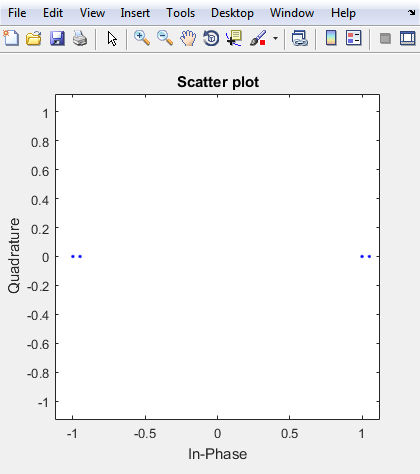
\includegraphics[width=0.95\textwidth]{bpsk}
\captionsetup{justification=centering,margin=1.0 cm}
\caption{Binary Phase Shift Keying map}
\label{any}
\end{figure}

Можно изменить параметр M в модуляции PSK на 4 и получить QPSK (Quadratic), или на 8 и получить 8-PSK:

\begin{figure}[H]
\centering
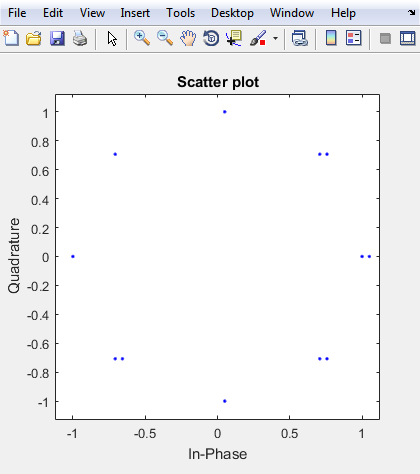
\includegraphics[width=0.95\textwidth]{8psk}
\captionsetup{justification=centering,margin=1.0 cm}
\caption{8-PSK map}
\label{any}
\end{figure}

Рассмотрим Minimum Shift Key модуляцию c параметром SamplesPerSymbol = 7:

\begin{figure}[H]
\centering
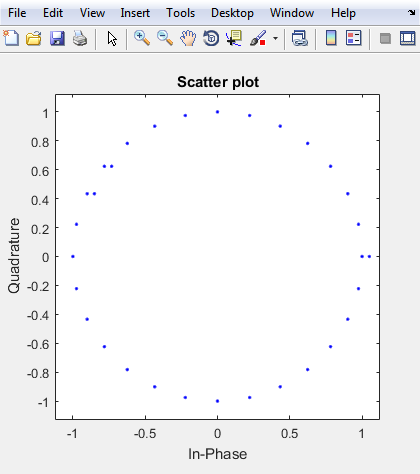
\includegraphics[width=0.95\textwidth]{msk}
\captionsetup{justification=centering,margin=1.0 cm}
\caption{Minimum Shift Key map (SPS = 7)}
\label{any}
\end{figure}

Наконец рассмотрим Offset Quadrature Phase Shift Keying modulation.

\begin{figure}[H]
\centering
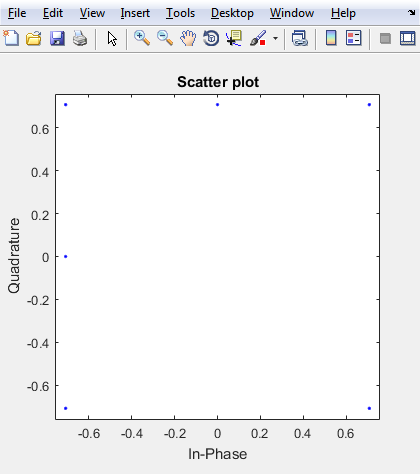
\includegraphics[width=0.95\textwidth]{oqpsk}
\captionsetup{justification=centering,margin=1.0cm}
\caption{OQPSK}
\label{sig}
\end{figure}

Не смотря на то, что модуляция четырехфазная, результатом модуляции являются комплексные числа.

\vspace{8cm}

\section{Выводы.}

В данной работе мы изучили различные виды фазовой, частотной и амплитудной модуляции цифровых сигналов:
\begin{itemize}

\item В фазовой модуляции PSK фаза несущего колебания имеет фиксированные позиции с одинаковым шагом, соответствующие цифровой посылке. С этим видом модуляции возникают проблемы синхронизации из-за трудности однозначной интерпретации поворота созвездия.

\item Квадратурная амплитудная модуляция характеризуется изменением и фазы, и амплитуды, из-за чего растёт информационная плотность.

\item Модуляция с минимальным сдвигом является примером частотной манипуляции, в ней нет фазовых ступеней, а частота изменяется в момент пересечения несущей нулевого уровня.

\item Бинарный PSK хоть и имеет низкую плотность информации ввиду всего двух ступеней фаз, но обладает большой помехоустойчивостью благодаря большой дистанции между этими двумя состояниями.
\end{itemize}


\end{document}
